\documentclass[aspectratio=169]{beamer}

\usepackage{graphicx}
\usepackage{minted}
\usemintedstyle{trac}

\setbeamertemplate{navigation symbols}{} % remove navigation symbols
\usefonttheme[onlymath]{serif} % beamer math looks like article math
\setbeamertemplate{frametitle continuation}{} % remove roman numerals created by framebreaks

\newcommand\vitem{\vfill\item}
\newcommand\pvitem{\pause\vfill\item}
\newcommand\pitem{\pause\item}

\newcommand\chighlight[2]{\setlength{\fboxsep}{0pt}\colorbox{#1}{#2\strut}}

\usetheme{Berlin}
% \setbeamertemplate{footline}[frame number]{}
\setbeamertemplate{headline}{}
\renewcommand{\insertnavigation}[1]{}

\title[]{Towards Producing Shorter Congruence Closure Proofs in a State-of-the-art SMT Solver (Extended Abstract)}
\author{\emph{Bruno Andreotti}, Haniel Barbosa, Oliver Flatt}
\institute{}
\date{PAAR 2024 at Nancy, France, 2024--07--02}

\begin{document}

\begin{frame}
  \titlepage
\end{frame}

\begin{frame}{Congruence closure}
  \begin{itemize}
    \item The property of congruence states that, for any terms $x$, $y$, and
    any function $f$,
    $$x = y \rightarrow f(x) = f(y)$$
    \vitem For a given set of equalities, the congruence closure is a minimal
    equivalence relation that satisfies them, as well as reflexivity, symmetry,
    transitivity and \emph{congruence}
  \end{itemize}
\end{frame}

\begin{frame}{Congruence closure in SMT solvers}
  \begin{itemize}
    \item Congruence closure algorithms are essential for solving the theory of
    equality and uninterpreted functions (EUF)
    \vitem The solver will provide a a set of equalities and inequalities, and
    the congruence closure algorithm must determine if it is consistent
  \end{itemize}
\end{frame}

\begin{frame}{Congruence closure in SMT solvers}
  \begin{itemize}
    \item However, for SMT solvers, it is not sufficient to just determine
    whether two terms are equivalent
    \vitem We also require an \textit{explanation}, that is, a minimal set of
    equations that makes the terms equivalent
    \pvitem Furthermore, we might also want a structured \textit{proof}, that
    uses these equalities as assumptions to derive the equivalence of the two
    terms
  \end{itemize}
\end{frame}

\begin{frame}{Proof-producing congruence closure}
  \begin{itemize}
    \item A proof-producing congruence closure algorithm was presented by
    Nieuwenhuis et al. in 2005
    \vitem It is based on a union-find data structure, and contructs an equality
    graph to represent the equivalence relation
    \pvitem Then, finding the explanation for the equivalence of two terms
    consists in finding a path between them in the graph
  \end{itemize}
\end{frame}

% TODO: why small proofs are important for SMT solvers

\begin{frame}{Proof-producing congruence closure: Example}
  \begin{itemize}
    \item TODO
  \end{itemize}
\end{frame}

\begin{frame}{Keeping redundant equalities}
  \begin{itemize}
    \item You may have noticed that we discard equalities between terms we
    already know to be equivalent
    \vitem However, keeping these equalities might allow us to find shorter
    paths between terms, and thus sorter proofs
  \end{itemize}
\end{frame}

\begin{frame}{Keeping redundant equalities}
  \begin{itemize}
    \item Flatt et al. at FMCAD'22 presented two proof producing congruence
    closure algorithms that make use of redundant equalities to find smaller
    proofs
    \pvitem In the original work, they were implemented in an equality
    saturation tool
    \pvitem Here, we present our effort to implement these algorithms in cvc5, a
    state-of-the-art SMT solver
  \end{itemize}
\end{frame}

\begin{frame}{Keeping redundant equalities: Example}
  \begin{itemize}
    \item TODO
  \end{itemize}
\end{frame}

\begin{frame}{A side note: tree-size vs DAG-size}
  \begin{itemize}
    \item Finding the minimal proof for the equivalence of two terms is an
    NP-hard problem
    \vitem However, this problem becomes easier if we don't allow the reuse of
    proof steps
    \pvitem We call this the \emph{tree size} of the proof, in contrast to the
    \emph{DAG size}
  \end{itemize}
\end{frame}

\begin{frame}{\textsc{TreeOpt} algorithm}
  \begin{itemize}
    \item Optimal algorithm (with regards to proof tree size)
    \vitem Computes the weight of each congruence edge by finding the size of
    the explanation of its justification, until a fixed point
    \vitem When asked to explain the equivalence between two terms, simply finds
    the sortest path between them considering these weights
  \end{itemize}
\end{frame}

\begin{frame}[fragile]{\textsc{TreeOpt} algorithm}
  \begin{minted}[autogobble=true, fontsize=\footnotesize]{js}
    function compute_weights():
        let weights = {}
        for edge in edges:
            if not edge.is_congruence_edge():
                weights[l, r] = 1

        until fixed point:
            for (l, r) in congruence_edges:
                weights[l, r] = find_shortest_path(l, r, weights).size()
        return weights
  \end{minted}
\end{frame}

\begin{frame}[fragile]{\textsc{TreeOpt} algorithm}
  \begin{minted}[autogobble=true, fontsize=\footnotesize]{js}
    function get_explanation(start, end, weights=compute_weights()):
        let explanation = []
        let path = find_shortest_path(start, end, weights)
        for edge in path:
            if edge.is_congruence_edge():
                let (j1, j2) = edge.justification()
                explanation += get_explanation(j1, j2, weights)
            else:
                explanation += edge
        return explanation
  \end{minted}
\end{frame}

\begin{frame}{\textsc{Greedy} algorithm}
  \begin{itemize}
    \item First, estimates the proof size of each congruence edge
    \vitem To explain the equivalence between two terms, finds the sortest path
    between them using these estimates as edge weights, but recurses when it
    encounters a congruence edge
  \end{itemize}
\end{frame}

\begin{frame}[fragile]{\textsc{Greedy} algorithm}
  \begin{minted}[autogobble=true, fontsize=\footnotesize, escapeinside=||]{js}
    function compute_weights():
        let weights = {}
        for edge in edges:
            if edge.is_congruence_edge():
                weights[l, r] = 1
            else:
                weights[l, r] = unoptimized_explanation(l, r).size()

        return weights
  \end{minted}
\end{frame}

\begin{frame}[fragile]{\textsc{Greedy} algorithm}
  \begin{minted}[autogobble=true, fontsize=\footnotesize, escapeinside=||]{js}
    function get_explanation(start, end, weights=compute_weights(), |\chighlight{green!30}{fuel}|):
        |\chighlight{green!30}{if fuel == 0:}|
        |\chighlight{green!30}{    return unoptimized\_explanation(start, end)}|

        let explanation = []
        let path = find_shortest_path(start, end, weights)
        for edge in path:
            if edge.is_congruence_edge():
                let (j1, j2) = edge.justification()
                explanation += get_explanation(j1, j2, |\chighlight{green!30}{fuel - 1}|)
            else:
                explanation += edge

        return explanation
  \end{minted}
\end{frame}

\begin{frame}{Dealing with backtracking}
  \begin{itemize}
    \item Modern SMT solvers work by trying many possible (partial) solutions,
    and backtracking when a solution is determined to be invalid
    \vitem So, a congruence closure algorithm must be able to efficiently revert
    to a previous state when backtracking
  \end{itemize}
\end{frame}

\begin{frame}{Dealing with backtracking}
  \begin{itemize}
    \item In our case, this is done by carefully recording the steps the
    congruence closure engine did, and undoing them when backtracking
    \vitem This includes clearing any cache that became invalid because of
    the backtrack (e.g., the \textsc{TreeOpt} and \textsc{Greedy} edge weights)
  \end{itemize}
\end{frame}

\begin{frame}{Avoiding circular explanations}
  \begin{itemize}
    \item When we were discarding redundant equalities, there could never be a
    redundant explanation
    \vitem This is because, after a congruence edge is added, the path between
    the terms of its justification will not change anymore
    \pvitem Now that we keep redundant edges, this is not true anymore
  \end{itemize}
\end{frame}

\begin{frame}{Avoiding circular explanations: Example}
  \begin{itemize}
    \item TODO
  \end{itemize}
\end{frame}

\begin{frame}{Avoiding circular explanations}
  \begin{itemize}
    \item To prevent this problem, we store in each edge the \emph{level} in
    which it was added
    \vitem Then, when explaining a congruence edge that was added in level $n$,
    we can only use edges whose level is no greater than $n$
  \end{itemize}
\end{frame}

\begin{frame}{Evaluation}
  \begin{itemize}
    \item TODO
  \end{itemize}
\end{frame}

\begin{frame}{Results}
  \begin{minipage}[c][0.5 \textheight]{0.3 \textwidth}
  \begin{itemize}
    \item Average runtime overhead was\\1.18x for \textsc{Greedy},\\2.68x
    for \textsc{TreeOpt}
  \end{itemize}
  \end{minipage}
  \hfill
  \begin{minipage}{0.68 \textwidth}
  \centerline{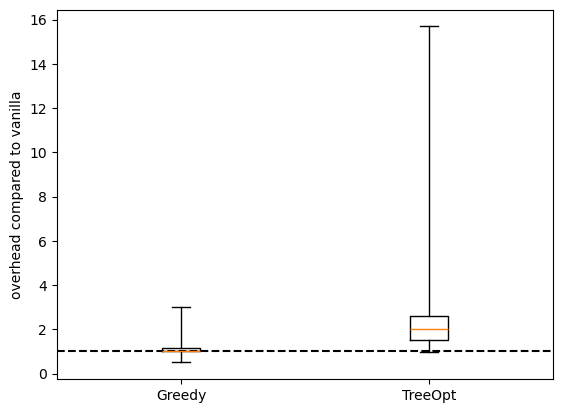
\includegraphics[width=\textwidth]{images/runtime-boxplot.png}}
  \end{minipage}
\end{frame}

\begin{frame}{Results}
  \begin{itemize}
    \item The new algorithms had no meaningful overall impact in the final proof
    size
    \vitem On average the proofs from \textsc{Greedy} and \textsc{TreeOpt} were
    0.2\% and 0.1\% larger that the \textsc{Vanilla} proofs
    \vitem They were 80\% smaller than the \textsc{Vanilla} proofs in the best
    case, and 70\% bigger in the worst case
  \end{itemize}
\end{frame}

\begin{frame}{Results}
  \begin{itemize}
    \item We also measured the size of the proof returned by each call to
    \texttt{get\_explanation}
    \vitem In 83\% of cases, the proofs returned by the three algorithms had the
    same size
    \vitem On average, the ``local'' proofs from the two new algorithms are 2\%
    smaller than the \textsc{Vanilla} proofs
    \pvitem If we exclude identical proofs, they are on average 14\% smaller
  \end{itemize}
\end{frame}

\begin{frame}{Results}
  \centerline{
  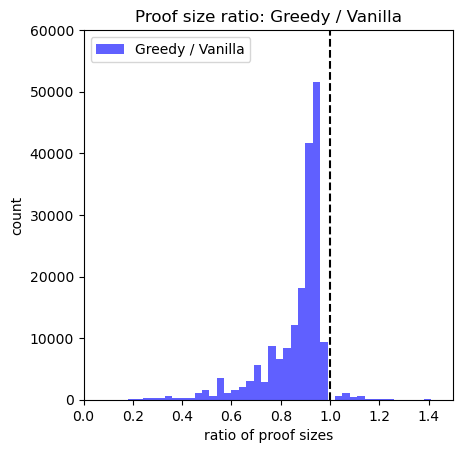
\includegraphics[width=0.45 \textwidth]{images/proof-ratio-hist-greedy.png}
  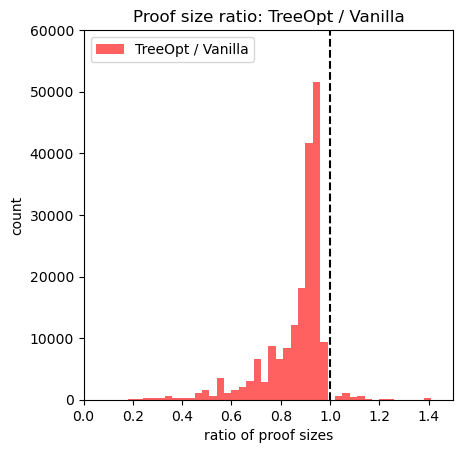
\includegraphics[width=0.45 \textwidth]{images/proof-ratio-hist-treeopt.png}
  }
\end{frame}

\begin{frame}{Results}
  \begin{minipage}[c][0.5 \textheight]{0.46 \textwidth}
  \begin{itemize}
    \item We also measured the number of redundant equalities added
    \vitem On average, 8.7\% of the equality graph edges were redundant, and in
    the most extreme case, 44.63\%
  \end{itemize}
  \end{minipage}
  \hfill
  \begin{minipage}{0.52 \textwidth}
  \centerline{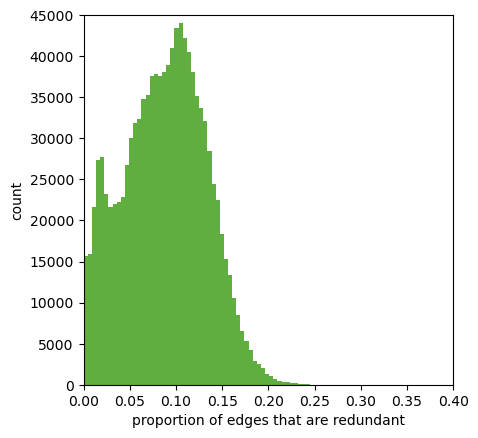
\includegraphics[width=\textwidth]{images/extra-hist.png}}
  \end{minipage}
\end{frame}

\begin{frame}{Conclusion}
  \begin{itemize}
    \item TODO
  \end{itemize}
\end{frame}

\end{document}
